\documentclass[aspectratio=169]{beamer}
\usetheme{Perso}

\usepackage[outputdir=build]{minted}
\setminted{breaklines}
\newminted{text}{frame=single}
\usemintedstyle{tango}
\graphicspath{ {images/} }


\title{The Lean Startup}
\date{\today}
\author{Maxime Vidori}

\begin{document}

\begin{frame}
  \titlepage
\end{frame}

\begin{frame}{Intro}
  \pause
  \Large \textbf{Why startups fail?} \normalsize \\
  \pause
\begin{block}{Achieving failure}
    Successfully, faithfully rigorously executing a plan that turned out to have
     been utterly flawed.
  \end{block}
  \pause
  \begin{block}{"Just do it" school of startups}
    If management is the problem , chaos is the answer!
  \end{block}


\end{frame}

\note[itemize]{
\item simple question -> Why startups fails
\item nothing was paved and no rules seamed to
}

\begin{frame}{Vision}{Start}
  \begin{itemize}
    \item Cross-functional teams, accountable to what we call \textit{learning milestone}.
    \item The goal of a startup is to figure out the right thing to build.
  \end{itemize}
  \begin{figure}
    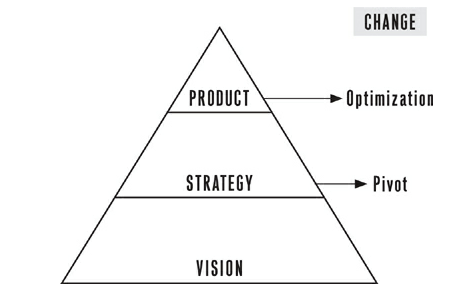
\includegraphics[scale=0.55]{LS_pyramid}
  \end{figure}

\end{frame}

\note[itemize]{
  \item Startups also have a true north, a destination in mind: creating a
    thriving and world-changing business. I call that a startup's vision.
}

\begin{frame}{Vision}{Define}
  \begin{block}{Entrepreneur}
    From young visionaries with little backing but great ideas to seasoned
    visionaries within larger companies.
  \end{block}
  \begin{block}{Startup}
    Human institution designed to create a new product or service under
    conditions of extreme uncertainty.
  \end{block}
\end{frame}

\note[itemize]{
\item entrepreneur, startup p27
}

\begin{frame}{Vision}{Learn}
\Large \textbf{Is my company is making progress toward creating a successful business?} \normalsize \\
\pause

  \begin{itemize}
    \item Measure $\rightarrow$ Validate learning.
    \item Value $/$ Waste.
    \item Example IMVU: throw a lot of work away (plugin, pivot).
  \end{itemize}
\end{frame}

\begin{frame}{Vision}{Experiment}
  \begin{columns}
    \begin{column}{0.5\textwidth}
  \begin{itemize}
      \item Think big, start small.
      \item An experiment is a product.
      \item Validate hypothesis.
  \end{itemize}
      \end{column}
\begin{column}{0.5\textwidth}  %%<--- here
   \begin{center}
     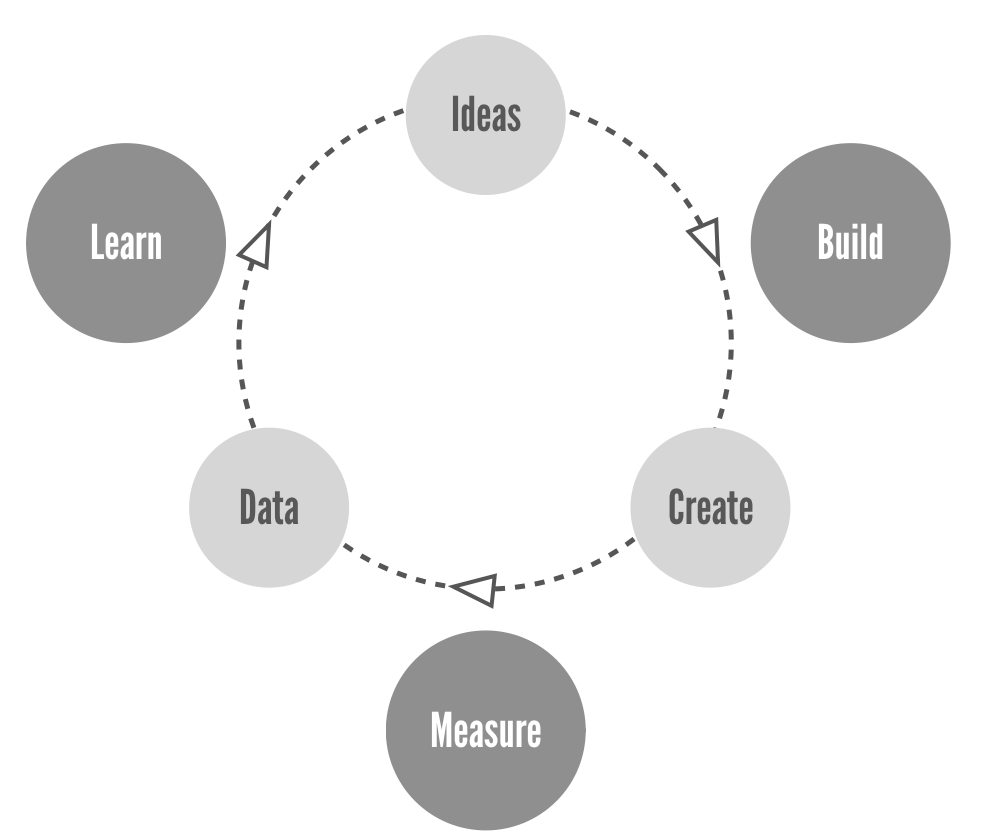
\includegraphics[scale=0.20]{build-measure-learn}
      \end{center}
\end{column}
  \end{columns}
\end{frame}

\note{
build, measure, learn feedback loop
}

\begin{frame}{Steer}{Leap}
  \begin{itemize}
    \item Strategy based on assumptions, two core hypothesis:
      \begin{enumerate}
        \item Value Hypothesis.
        \item Growth Hypothesis.
      \end{enumerate}

    \item Beyond "The right place at the right time".
    \item Value and growth,
    \item Genchi Gembuchu.
    \item Analysis paralysis.
  \end{itemize}
\end{frame}

\begin{frame}{Steer}{Test}
  \begin{itemize}
    \item Well known MVP's
      \begin{itemize}
        \item Groupon
        \item Dropbox
      \end{itemize}
    \item Different types of MVPs
      \begin{itemize}

        \item Video
        \item Concierge
        \item Wizard of Oz
      \end{itemize}
    \item Quality? $\rightarrow$ \textbf{Early adopters!}
  \end{itemize}
\end{frame}

\begin{frame}{Steer}{Measure}
  \begin{itemize}
    \item Three learning milestone:
      \begin{itemize}
        \item Establish the baseline.
        \item Tuning the engine.
        \item Pivot or persevere.
      \end{itemize}

    \item Product progress $\neq$ Business results.
    \item Vanity metrics $\rightarrow$ Cohort analysis.
    \item 3 A's: Actionable, Accessible, Auditable.
  \end{itemize}
\end{frame}

\begin{frame}{Steer}{Pivot or Persevere}
  \begin{itemize}
    \item Startup runway (number of pivots left).
    \item Pivot or persevere meeting.
    \item Pivot require courage $\rightarrow$ This is a strategic hypothesis.
    \item Famous pivots: Zoom-in, Zoom-out, Customer Segment, Engine of Growth, \ldots
  \end{itemize}
\end{frame}

\begin{frame}{Accelerate}{Batch}
  \begin{itemize}
    \item Lean Manufacturing: \textit{"single piece flow"}.
    \item Andon cord $\rightarrow$ Just in time production.
    \item Continuous Deployment.
    \item Large batch death spiral, silos organisation.
  \end{itemize}
\end{frame}

\begin{frame}{Accelerate}{Grow}
  \begin{itemize}
    \item 3 engines of growth:
      \begin{enumerate}
        \item \textbf{Sticky:} attract and retain customers.
        \item \textbf{Viral:} new customers attract new ones.
        \item \textbf{Paid:} company pays to attract new people (traditional).
      \end{enumerate}
    \item Engine of growth determine metrics to watch, and product/market fit.
  \end{itemize}
\end{frame}

\note[itemize]{
\item viral -> facebook, hotmail, tupperware
\item product/market fit -> there is customers for your product. If there is no
  market for your product, no matter how good your product or team is good, you
  are doomed.
}

\begin{frame}{Accelerate}{Adapt}
  \begin{itemize}
    \item 5 Why's $\rightarrow$ Natural speed regulator.
      \begin{itemize}
        \item Be tolerant of all mistakes the first time.
        \item Never allow the same mistake to be made twice.
      \end{itemize}
    \item Employees get more creative if fear of risks go down.
    \item Example: writing documentation.
  \end{itemize}
\end{frame}

\note[itemize]{
\item regulator: p233
}

\begin{frame}{Accelerate}{Innovate}
  \begin{itemize}
    \item Becoming the status quo.
    \item Creating an innovation sandbox.
    \item Do not hide innovation inside the Black Box.
    \item Holding internal teams accountable $\rightarrow$ a product team can be
      seen as a startup.
  \end{itemize}
\end{frame}

\begin{frame}{Epilogue}{Waste Not}
  \begin{itemize}
    \item \textbf{DANGER:} Putting the system first.
    \item Product Development PseudoScience.
    \item Evaluating manager on \textit{"vanity"} metrics.
  \end{itemize}
\end{frame}

\note[itemize]{
\item product development p278: Green light based on intuition than facts
\item LTSE: 282
}
\begin{frame}{That's all folks}
  \LARGE \textbf{Questions?}

  \begin{flushright}
    \normalsize github.com/\color{Green}IxDay\color{Grey}/talks/the-lean-startup
   \end{flushright}
\end{frame}


\end{document}
